\fancyhead[RO]{\fontsize{8.5pt}{10pt}\selectfont\textbf{\textsf{MỤC 1.2}}\quad \textsf{Mô hình toán học: Danh mục các hàm số cơ bản}\quad \textbf{\textsf{35}}}
\fancyhead[LE]{\fontsize{8.5pt}{10pt}\selectfont\textbf{\textsf{35}}\quad \textbf{\textsf{CHƯƠNG 1}}\quad \textsf{Hàm số và Mô hình}}

\noindent
\begin{minipage}[t]{0.485\textwidth}
    \fontsize{9pt}{12.5pt}\selectfont
    \noindent đo bằng oát (W) và $T$ là nhiệt độ tuyệt đối đo bằng kenvin (K).
    \begin{enumerate}[label=\textbf{(\alph*)}, leftmargin=*, itemsep=1pt, topsep=2pt]
        \item Vẽ đồ thị hàm số $E$ theo nhiệt độ $T$ trong khoảng từ $100\text{ K}$ đến $300\text{ K}$.
        \item Dùng đồ thị để mô tả sự thay đổi của năng lượng $E$ khi nhiệt độ $T$ tăng dần.
    \end{enumerate}

    \vspace{6pt}
    \noindent\textbf{\color{stewartcyan}27--28}\quad Với mỗi biểu đồ phân tán dưới đây, hãy xác định loại hàm số nào bạn có thể chọn làm mô hình cho dữ liệu. Giải thích sự lựa chọn của bạn.

    \vspace{8pt}
    \noindent\textbf{27.}
    \begin{center}
    \begin{minipage}[t]{0.46\linewidth}
        \centering
        \textbf{(a)}\\[2pt]
        \begin{tikzpicture}[scale=0.85, baseline=(current bounding box.center)]
            \draw[->, >=stealth] (-0.2,0) -- (2.5,0) node[below] {$x$};
            \draw[->, >=stealth] (0,-0.2) -- (0,2.1) node[left] {$y$};
            \node[below left] at (0,0) {$0$};
            \foreach \x/\y in {
                0.2/1.65, 0.3/1.42, 0.4/1.22, 0.5/0.95, 0.6/0.82, 0.7/0.95, 0.8/1.20,
                0.9/1.42, 1.0/1.65, 1.1/1.62, 1.2/1.45, 1.3/1.20, 1.4/0.95, 1.5/0.85,
                1.6/1.02, 1.7/1.30, 1.8/1.62, 1.9/1.66, 2.0/1.48
            } {
                \fill[stewartcyan] (\x,\y) circle (1.2pt);
            }
        \end{tikzpicture}
    \end{minipage}\hfill
    \begin{minipage}[t]{0.46\linewidth}
        \centering
        \textbf{(b)}\\[2pt]
        \begin{tikzpicture}[scale=0.85, baseline=(current bounding box.center)]
            \draw[->, >=stealth] (-0.2,0) -- (2.5,0) node[below] {$x$};
            \draw[->, >=stealth] (0,-0.2) -- (0,2.1) node[left] {$y$};
            \node[below left] at (0,0) {$0$};
            \foreach \x/\y in {
                0.15/1.85, 0.25/1.72, 0.35/1.78, 0.45/1.60, 0.55/1.52, 0.65/1.45, 0.75/1.48,
                0.85/1.32, 0.95/1.38, 1.05/1.22, 1.15/1.28, 1.25/1.12, 1.35/1.05, 1.45/0.92,
                1.55/0.98, 1.65/0.82, 1.75/0.74, 1.85/0.78, 1.95/0.65, 2.05/0.52, 2.15/0.58,
                2.25/0.42, 2.35/0.32
            } {
                \fill[stewartcyan] (\x,\y) circle (1.2pt);
            }
        \end{tikzpicture}
    \end{minipage}
    \end{center}

    \vspace{4pt}
    \noindent\textbf{28.}
    \begin{center}
    \begin{minipage}[t]{0.46\linewidth}
        \centering
        \textbf{(a)}\\[2pt]
        \begin{tikzpicture}[scale=0.85, baseline=(current bounding box.center)]
            \draw[->, >=stealth] (-0.2,0) -- (2.5,0) node[below] {$x$};
            \draw[->, >=stealth] (0,-0.2) -- (0,2.1) node[left] {$y$};
            \node[below left] at (0,0) {$0$};
            \foreach \x/\y in {
                0.15/0.45, 0.35/0.40, 0.50/0.50, 0.65/0.60, 0.80/0.70, 0.90/0.75,
                1.00/0.90, 1.10/1.05, 1.20/1.20, 1.30/1.42, 1.35/1.65, 1.40/1.85
            } {
                \fill[stewartcyan] (\x,\y) circle (1.2pt);
            }
        \end{tikzpicture}
    \end{minipage}\hfill
    \begin{minipage}[t]{0.46\linewidth}
        \centering
        \textbf{(b)}\\[2pt]
        \begin{tikzpicture}[scale=0.85, baseline=(current bounding box.center)]
            \draw[->, >=stealth] (-0.2,0) -- (2.5,0) node[below] {$x$};
            \draw[->, >=stealth] (0,-0.2) -- (0,2.1) node[left] {$y$};
            \node[below left] at (0,0) {$0$};
            \foreach \x/\y in {
                0.20/1.95, 0.25/1.70, 0.30/1.45, 0.35/1.10, 0.45/0.85, 0.55/0.75,
                0.70/0.65, 0.85/0.55, 1.05/0.48, 1.25/0.42, 1.50/0.38, 1.75/0.35,
                2.00/0.32, 2.20/0.30, 2.35/0.32
            } {
                \fill[stewartcyan] (\x,\y) circle (1.2pt);
            }
        \end{tikzpicture}
    \end{minipage}
    \end{center}

    \vspace{6pt}
    \noindent\tikz[baseline=-0.6ex]\node[fill=stewartcyan,text=white,inner sep=1.2pt,rounded corners=0.5pt]{\fontsize{7.5pt}{7.5pt}\selectfont\textbf{\textsf{T}}}\;\textbf{29.} Bảng dưới đây cho thấy tỉ lệ mắc bệnh loét dạ dày tá tràng (suốt đời) (trên 100 người dân) ứng với các mức thu nhập hộ gia đình khác nhau, theo báo cáo của Khảo sát Phỏng vấn Y tế Quốc gia.
    \begin{enumerate}[label=\textbf{(\alph*)}, leftmargin=*, itemsep=1.5pt, topsep=2pt]
        \item Vẽ biểu đồ phân tán của tập dữ liệu này và cho biết liệu mô hình tuyến tính có phù hợp hay không.
        \item Tìm và vẽ đồ thị mô hình tuyến tính sử dụng điểm dữ liệu đầu tiên và điểm dữ liệu cuối cùng.
        \item Tìm và vẽ đồ thị đường hồi quy.
        \item Dùng mô hình tuyến tính ở câu (c) để ước tính tỉ lệ loét dạ dày ở những người có mức thu nhập \$25.000.
        \item Theo mô hình, khả năng một người có thu nhập \$80.000 bị loét dạ dày tá tràng là bao nhiêu?
        \item Bạn có nghĩ việc áp dụng mô hình này cho một người có thu nhập \$200.000 là hợp lý không?
    \end{enumerate}

    \begin{center}
        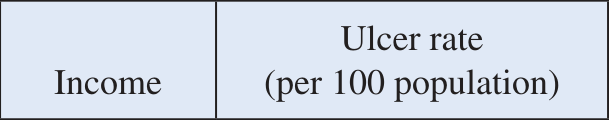
\includegraphics[width=0.72\linewidth]{images/p0070_graph_3.png}
    \end{center}
\end{minipage}%
\hfill
\begin{minipage}[t]{0.485\textwidth}
    \fontsize{9pt}{12.5pt}\selectfont
    \noindent\tikz[baseline=-0.6ex]\node[fill=stewartcyan,text=white,inner sep=1.2pt,rounded corners=0.5pt]{\fontsize{7.5pt}{7.5pt}\selectfont\textbf{\textsf{T}}}\;\textbf{30.} Khi chuột trong phòng thí nghiệm tiếp xúc với sợi amiăng, một số con xuất hiện khối u phổi. Bảng bên dưới liệt kê kết quả của một số thí nghiệm do các nhà khoa học khác nhau thực hiện.
    \begin{enumerate}[label=\textbf{(\alph*)}, leftmargin=*, itemsep=1.5pt, topsep=2pt]
        \item Tìm đường hồi quy cho dữ liệu.
        \item Vẽ biểu đồ phân tán và vẽ đồ thị đường hồi quy. Đường hồi quy có vẻ là một mô hình thích hợp cho tập dữ liệu không?
        \item Giao điểm với trục tung ($y$-intercept) của đường hồi quy biểu diễn điều gì?
    \end{enumerate}

    \begin{center}
        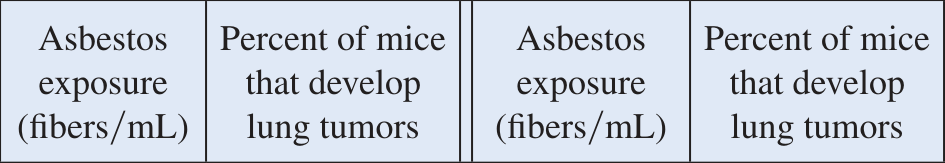
\includegraphics[width=0.98\linewidth]{images/p0070_graph_1.png}
    \end{center}

    \vspace{4pt}
    \noindent\tikz[baseline=-0.6ex]\node[fill=stewartcyan,text=white,inner sep=1.2pt,rounded corners=0.5pt]{\fontsize{7.5pt}{7.5pt}\selectfont\textbf{\textsf{T}}}\;\textbf{31.} Các nhà nhân chủng học sử dụng một mô hình tuyến tính liên hệ chiều dài xương đùi của con người với chiều cao cơ thể. Mô hình này cho phép nhà nhân chủng học xác định chiều cao của một cá nhân khi chỉ tìm thấy một phần bộ xương (bao gồm xương đùi). Ở đây chúng ta tìm mô hình bằng cách phân tích dữ liệu về chiều dài xương đùi và chiều cao của tám người nam giới cho trong bảng.
    \begin{enumerate}[label=\textbf{(\alph*)}, leftmargin=*, itemsep=1.5pt, topsep=2pt]
        \item Vẽ biểu đồ phân tán của dữ liệu.
        \item Tìm và vẽ đồ thị đường hồi quy mô hình hóa dữ liệu.
        \item Một nhà nhân chủng học tìm thấy một xương đùi người dài 53 cm. Người đó cao bao nhiêu?
    \end{enumerate}

    \begin{center}
        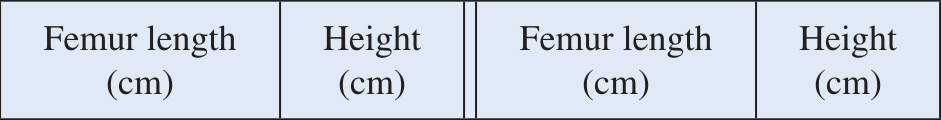
\includegraphics[width=0.98\linewidth]{images/p0070_graph_2.png}
    \end{center}

    \vspace{4pt}
    \noindent\tikz[baseline=-0.6ex]\node[fill=stewartcyan,text=white,inner sep=1.2pt,rounded corners=0.5pt]{\fontsize{7.5pt}{7.5pt}\selectfont\textbf{\textsf{T}}}\;\textbf{32.} Bảng dưới đây cho thấy giá bán lẻ điện trung bình tại Hoa Kỳ từ năm 2000 đến 2016, tính theo cent trên mỗi kilowatt-giờ.
    \begin{enumerate}[label=\textbf{(\alph*)}, leftmargin=*, itemsep=1.5pt, topsep=2pt]
        \item Vẽ biểu đồ phân tán. Mô hình tuyến tính có phù hợp không?
        \item Tìm và vẽ đồ thị đường hồi quy.
        \item Sử dụng mô hình tuyến tính ở câu (b) để ước lượng giá bán lẻ điện trung bình vào năm 2005 và 2017.
    \end{enumerate}

    \begin{center}
        \renewcommand{\arraystretch}{1.12}
        \setlength{\tabcolsep}{4pt}
        \begin{tabular}{|c|c||c|c|}
            \hline
            \rowcolor{stewarttablehead!60}
            \textsf{Số năm kể từ 2000} & \textsf{Cents/kWh} & \textsf{Số năm kể từ 2000} & \textsf{Cents/kWh} \\
            \hline
            0 & 8{,}24 & 10 & 11{,}54 \\
            2 & 8{,}44 & 12 & 11{,}88 \\
            4 & 8{,}95 & 14 & 12{,}52 \\
            6 & 10{,}40 & 16 & 12{,}90 \\
            8 & 11{,}26 & & \\
            \hline
        \end{tabular}
        \\[3pt]
        {\fontsize{7.5pt}{9pt}\selectfont\textit{Nguồn:} Cơ quan Thông tin Năng lượng Hoa Kỳ (US Energy Information Administration)}
    \end{center}
\end{minipage}